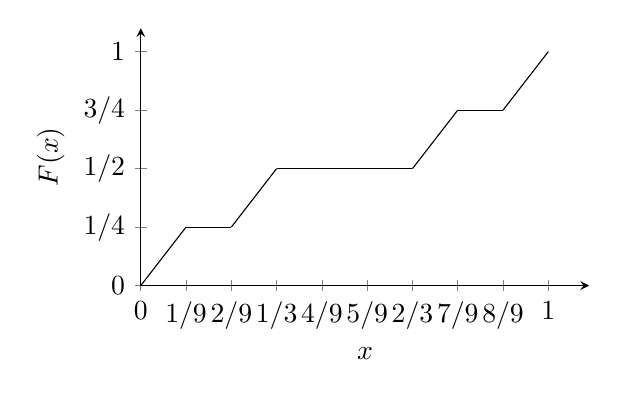
\begin{tikzpicture}
    \begin{axis}[
    axis lines=left,
    xlabel = $x$, ylabel = $F(x)$,
    xmax = 1.1, xtick = {0, 1/9, 2/9, 3/9, 4/9, 5/9, 6/9, 7/9, 8/9, 1}, 
    ymax = 1.1, ytick = {0, 1/4, 1/2, 3/4, 1},
    xticklabels={$0$, $1/9$, $2/9$, $1/3$, $4/9$, $5/9$, $2/3$, $7/9$, $8/9$, $1$},
    yticklabels={$0$, $1/4$, $1/2$, $3/4$, $1$}, 
    width=0.6\textwidth, height=0.4\textwidth]
    \addplot[domain=0:1/9] {9*x/4};
    \addplot[domain=1/9:2/9] {1/4};
    \addplot[domain=2/9:1/3] {9*(x-1/3)/4 + 1/2};
    \addplot[domain=1/3:2/3] {1/2};
    \addplot[domain=2/3:7/9] {9*(x-7/9)/4 + 3/4};
    \addplot[domain=7/9:8/9] {3/4};
    \addplot[domain=8/9:1] {9*(x-1)/4 + 1};
    \end{axis}
\end{tikzpicture}